\section{建模与求解}
% 简单陈述主要内容, 比如
% 这里将通过数学建模,讨论\解决本文所提出的X个问题。共分为X个小节。
% 或者
% 在这里,讨论本文所提出的X个问题解答,对每个问题分别进行数学建模与模型求解。共分为X个小节。
这里将通过数学建模,讨论并解决本文所提出的 X 个问题。共分为 X 个小节。

\subsection{问题一的建模与求解}
% 简短的概述, 问题一主要要解决什么问题, 建立了××××××模型, 用了什么方法解决. 
% 写出本小节主要内容(比如:本小节主要内容是数据的预处理、××××××模型的建立、模型的求解和分析、模型检验). 
问题一主要解决 ×××××× 问题,为此建立了 ×××××× 模型, 采用了 ×××××× 方法进行求解。
本小节主要内容包括:数据的预处理、××××××模型的建立、模型的求解和分析、模型检验或修正。

\subsubsection{数据的预处理(如果是做数据多的题, 一定要写这一块; 不需要的就不做.)}
    \textbf{1. 数据的采集}
    
    ××××××××
    
    \textbf{2. 去噪处理}
    
    ××××××××
    
    \textbf{3. 数据的整理(如不全的数据要补全, 有的是要转化数据类型, 等等)}
    
    ××××××××

\begin{figure}[H] % [H] 选项来自 float 宏包,表示将图片"确实放在这里"
    \centering      % 图片居中显示
    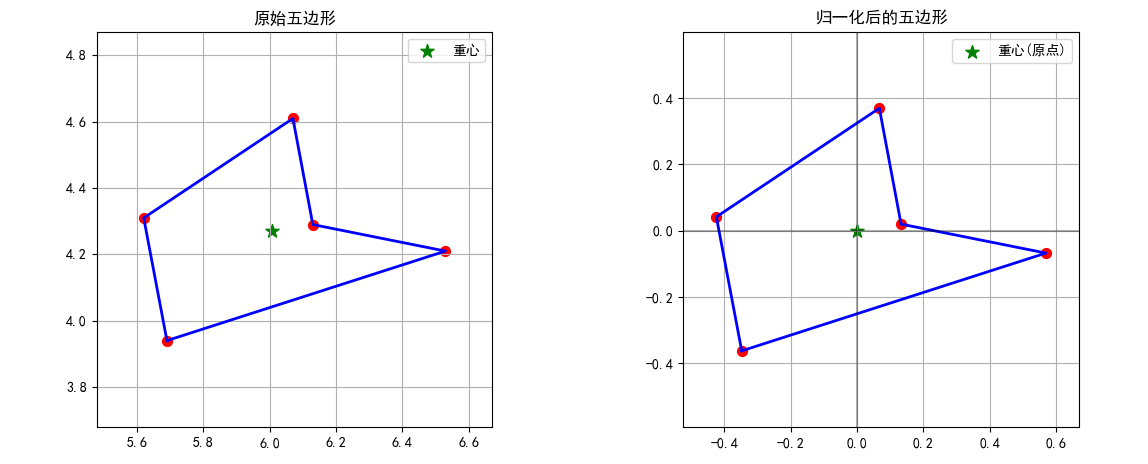
\includegraphics[width=1\textwidth]{figures/pentagon_normalization.png}

    % 说明:
    % 1. figures/pentagon_normalization.png 是您的图片文件相对于 .tex 文件的路径。
    % 2. [width=0.8\textwidth] 是一个可选参数,用于设置图片的宽度。
    %    0.8\textwidth 表示图片宽度为当前文本宽度的 80%。
    %    您可以根据需要调整这个值。
    \caption{xxx示例}
    \label{fig:normalize} % \label 必须放在 \caption 之后或内部,以便正确引用
\end{figure}

\subsubsection{xxxx模型的建立}

% 注意, 模型一般是数学公式, 少数情况可以是图形(常用图论求解时会用到)+一个算法(算法要写伪算法或给出流程图). 
% 但不能是纯文字说明. 下附算法的模板供参考. 在建模的过程,应该有必要的推理、推导、演算等. 
% 模型建立的叙述非常重要, 同学们往往是思路有了, 却怎么也交代不清楚,甚至觉得无话可说. 
% 大家要多看, 多写, 多思考才能写好. 我建模组老师也会尽量做到多给大家修改.
% 多看: 就是要多看优秀论文, 模仿优秀作品的写法先.
% 多练: 就是要多做题, 写完整的论文. 练一次, 写作能力就会提高一级.
% 多想: 就是要想想别人的文章好, 自己的不好, 差距在哪里?别人的文章还能不能改进, 写得更好. 
% 如果是几个模型, 采用格式:
% 1. ××××××模型
% ××××××××
% 2. ××××××模型
% ××××××××
% 3. ××××××模型
% ××××××××
在此处描述模型的建立过程,包括必要的推理、推导、演算等。
例如,可以定义模型的目标函数、约束条件等:
\begin{equation}
    \min f(x) = \sum_{i=1}^{n} c_i x_i \label{eq:obj_func_q1}
\end{equation}
约束条件:
\begin{align}
    \sum_{j=1}^{m} a_{ij} x_j \leq b_i, \quad & \forall i = 1, \dots, k \\
    x_j \geq 0, \quad & \forall j = 1, \dots, m
\end{align}
% 如果有算法,请使用伪代码或流程图描述。

\begin{algorithm}[H] % [H] 选项来自 float 宏包
\caption{五边形归类判别算法}
\label{alg:polygon_classification}
\begin{algorithmic}[1] % [1] 表示显示行号
    \Function{ClassifyPolygon}{$P, \mathit{ClassI}, \mathit{ClassII}$}
        \State 对输入的待测五边形$P$、类别I模板$\mathit{ClassI}$、类别II模板$\mathit{ClassII}$进行归一化处理
        \State 提取$P$的几何不变量特征向量$\mathcal{F}_P$
        \State 提取$\mathit{ClassI}$的几何不变量特征向量$\mathcal{F}_I$
        \State 提取$\mathit{ClassII}$的几何不变量特征向量$\mathcal{F}_{II}$
        \State 计算$P$与$\mathit{ClassI}$的特征向量欧氏距离 $d_{\mathcal{F},I} = \|\mathcal{F}_P - \mathcal{F}_I\|_2$
        \State 计算$P$与$\mathit{ClassII}$的特征向量欧氏距离 $d_{\mathcal{F},II} = \|\mathcal{F}_P - \mathcal{F}_{II}\|_2$
        \State 尝试所有可能的顶点对应和旋转,使用Kabsch算法计算$P$与$\mathit{ClassI}$和$\mathit{ClassII}$之间的最优刚性配准,得到$\mathit{RMSD}_{I}$和$\mathit{RMSD}_{II}$
        \State 计算$P$与$\mathit{ClassI}$的综合相似度评分 $S_I = \alpha \cdot \mathit{RMSD}_I + (1-\alpha) \cdot d_{\mathcal{F},I}$ 
        \State 计算$P$与$\mathit{ClassII}$的综合相似度评分 $S_{II} = \alpha \cdot \mathit{RMSD}_{II} + (1-\alpha) \cdot d_{\mathcal{F},II}$
        \If{$S_I < S_{II}$ \textbf{and} $S_I < \lambda$} \Comment{$\lambda$为预设阈值}
            \State \Return 类别I
        \ElsIf{$S_{II} < S_I$ \textbf{and} $S_{II} < \lambda$}
            \State \Return 类别II
        \Else
            \State \Return 未知类别
        \EndIf
    \EndFunction
\end{algorithmic}
\end{algorithm}


\subsubsection{模型的求解和分析}
    
    \textbf{1. 计算方法的选取or设计}
    
    为解问题一××××××模型,主要采用了××××××××算法。
    % 比较复杂的程序要写算法或者流程图(但是不要在正文中出现代码,代码一律在附件里)。
    
    \textbf{2. 参数的确定}
    
    对所建模型中参数是如何确定的,写出过程和具体的值。例如
    确定上述公式(\ref{eq:obj_func_q1})中的参数见表\ref{tab:params_q1}. 
    % 需要自行创建该表格
    
   \begin{table}[H]
    \centering
    \caption{五边形归类结果}
    \label{tab:params_q1}
    % --- 使用混合列类型 ---
    \begin{tabularx}{\textwidth}{ c c c c c C c } %<-- 核心修改

    \toprule
    \textbf{图形编号} & \textbf{RMSD\textsubscript{I}} & \textbf{RMSD\textsubscript{II}} & \textbf{$d_{\mathcal{F},I}$} & \textbf{$d_{\mathcal{F},II}$} & \textbf{综合评分(I/II)} & \textbf{归类结果} \\
    \midrule
    1 & 0.0082 & 0.2956 & 0.3220 & 6.5186 & 0.0578 / 1.2782 & 类别I \\
    2 & 0.3010 & 0.0160 & 6.7958 & 0.4994 & 1.3265 / 0.0924 & 类别II \\
    3 & 0.1812 & 0.2235 & 4.4074 & 5.5873 & 0.8485 / 1.0704 & 未知类别 \\
    4 & 0.0101 & 0.2937 & 0.3142 & 6.5064 & 0.0581 / 1.2747 & 类别I \\
    5 & 0.3010 & 0.0489 & 7.8076 & 1.6174 & 1.4862 / 0.2965 & 类别II \\
    \bottomrule
    \end{tabularx}
\end{table}

    \textbf{3. 计算结果}
    
    将确定的参数代入模型(公式\ref{eq:obj_func_q1}),运用×××软件的什么命令, 或自己编写的程序(程序见附录×), 得到怎样的结果. 
    % (结果展示以表格和图为好)

    \textbf{4. 结果分析}
    
    从图×或表×可以看出:×××××××××××××××(单调性,极值,最值,拐点). 结论是什么(定性结果:变好、变坏,增加、减少).
    
    \textbf{5. 问题一的回答}
    
    利用计算结果,逐一回答问题一提出的每一个问题。对随时间变换的量,建议给出时间变换曲线图。


\subsubsection{模型检验或修正}
说明假设合理性,说明在前文的假设下结果的正确性(合理性), 诸如此类.可以通过对误差进行分析(如,做仿真模拟), 提出修改假设和对模型的修正。
××××××